%%% Lecture 1 Slides %%%

\documentclass{beamer}

%\documentclass[handout]{beamer}
%\usepackage{pgfpages}
%\pgfpagesuselayout{2 on 1}[a4paper,border shrink=5mm]
%\pgfpagesuselayout{1 on 1}[a4paper,border shrink=5mm]



\usepackage{amssymb}
\usepackage{amsmath}
\usepackage{mathtools}
\usepackage{tikz}
\usetikzlibrary{shapes,arrows}
\usetikzlibrary{positioning}
\usetikzlibrary{trees}
\usepackage{pgfplots}
\usepackage{pdflscape}
\usepackage{graphicx}
\usepackage{colortbl}
\usepackage{listings}
\usepackage{adjustbox}

\DeclarePairedDelimiter{\ceil}{\lceil}{\rceil}

\newcommand{\bs}{\boldsymbol}
\newcommand{\mb}{\mathbf}
\newcommand{\indep}{{\bot\negthickspace\negthickspace\bot}}
\newcommand{\notindep}{{\bot\negthickspace\negthickspace\bot}{\negthinspace
  \negmedspace \negthickspace \negthickspace \diagup
  \;}}
\renewcommand{\S}{\mb{S}}
\usepackage{color}
\definecolor{direct}{HTML}{FF0000}
\definecolor{indirect}{HTML}{FF9999}
\definecolor{dirin}{HTML}{990000}
\definecolor{control}{HTML}{999999}
\definecolor{directE}{HTML}{ED1C24}
\definecolor{indirectE}{HTML}{F69679}
\definecolor{controlE}{HTML}{999999}

%\defV{{\rm Var}\,}
\def\E{{\rm E}\,}
\def\arg{{\rm arg}\,}
\def\Cov{{\rm Cov}\,}
\def\N{{\rm N}\,}
\newcommand{\plim}{{\rm plim} \,}
\DeclareMathOperator*{\argmin}{arg\,min}
\newcommand{\X}{\mathbf{X}}
\newcommand{\Y}{\mathbf{Y}}
\newcommand{\Z}{\mathbf{Z}}
\newcommand{\I}{\mathbf{I}}
\newcommand{\V}{\mathbf{\Omega}}
\newcommand{\W}{\mathbf{W}}
\newcommand{\R}{\mathbf{R}}
\newcommand{\A}{\mathbf{A}}
\newcommand{\B}{\mathbf{B}}
\newcommand{\D}{\mathbf{D}}
\newcommand{\T}{\mathbf{T}}
\newcommand{\F}{\mathbf{F}}
\renewcommand{\O}{\mathbf{O}}
\renewcommand{\H}{\mathbf{H}}
\newcommand{\g}{\mathbf{g}}
\renewcommand{\r}{\mathbf{r}}
\newcommand{\s}{\mathbf{s}}
\newcommand{\uu}{\mathbf{u}}
\newcommand{\w}{\mathbf{w}}
\newcommand{\x}{\mathbf{x}}
\newcommand{\vv}{\mathbf{v}}
\newcommand{\z}{\mathbf{z}}
\newcommand{\y}{\mathbf{y}}

\newcommand{\bi}{\begin{itemize}}
\newcommand{\ei}{\end{itemize}}
\newcommand{\be}{\begin{enumerate}}
\newcommand{\ee}{\end{enumerate}}

\newcommand{\Beta}{\boldsymbol{\beta}}
\newcommand{\btheta}{\boldsymbol{\theta}}
\newcommand{\bgamma}{\boldsymbol{\gamma}}
\newcommand{\bpi}{\boldsymbol{\pi}}
\newcommand{\arrowp}{\stackrel{p}{\rightarrow}}
\newcommand{\arrowd}{\stackrel{d}{\rightarrow}}
\newcommand{\0}{\mathbf{0}}
\newcommand{\bP}{\mathbf{P}}
\newcommand{\nn}{\nonumber}
\def\S{{\sigma}}
\def\Supp{{\rm Supp}\,}


\newcommand\independent{\protect\mathpalette{\protect\independenT}{\perp}}
\def\independenT#1#2{\mathrel{\rlap{$#1#2$}\mkern2mu{#1#2}}}

\newcommand{\vsf}{\vspace{.5cm}}

\usepackage[english]{babel}
% or whatever

\usepackage[latin1]{inputenc}
% or whatever

\usepackage{times}
\usepackage[T1]{fontenc}
\setbeamertemplate{footline}[page number]{}
\setbeamertemplate{navigation symbols}{}


\title[Lecture 15] % (optional, use only with long paper titles)
{Lecture 15}


\begin{document}

\maketitle


%\frame{
%\frametitle{Linear Models: what are they good for?}
%
%Linear Models
%\begin{enumerate}
%\item Easy to fit
%\item Easy to interpret
%\item Nice properties (e.g., FWL)
%\item Easy SE formulas
%\item Easy sensitivity analysis (later)
%\end{enumerate}\pause
%
%\bigskip
%
%Non-linear Models
%\begin{enumerate}
%\item Easy to fit? (yep, computers)
%\item Easy to interpret? (kind of, computers)
%\item Nice properties (some, BDC later)
%\item Easy SE formulas? (no, but bootstrapping)
%\item Easy sensitivity analysis? (later) \pause
%\item Robust? (yep, computers and cross-validation)
%\end{enumerate}
%
%
%}


\frame{
\frametitle{Multiple Regression with Interactions and Polynomials}

\begin{itemize}
\item For the last few lectures we have focused on understanding, estimating and forming confidence intervals for OLS regression coefficients. \pause
\item As we include more polynomial terms and interaction terms, the beta coefficients may not be of direct interest. \pause
%\item Linear (with respect to the betas) regression can be made non-linear (with respect to the covariates) with the inclusion of polynomial terms.
\item With a binary covariate of interest and control variables including polynomials and interactions, the OLS regression produces two curves, two surfaces, or two hyper-surfaces. The estimate of interest in this case is often the average of the vertical distances between the curves, surfaces, etc. \pause
\item This average of vertical distances can be seen as an Average Partial Derivative, which can itself be extended to non-binary covariates of interest (with and without additional covariates). 
\end{itemize}

}


\frame{
\frametitle{Neto and Cox (1997) Table 3 Data}

\begin{figure}[ht]
  \begin{center}
    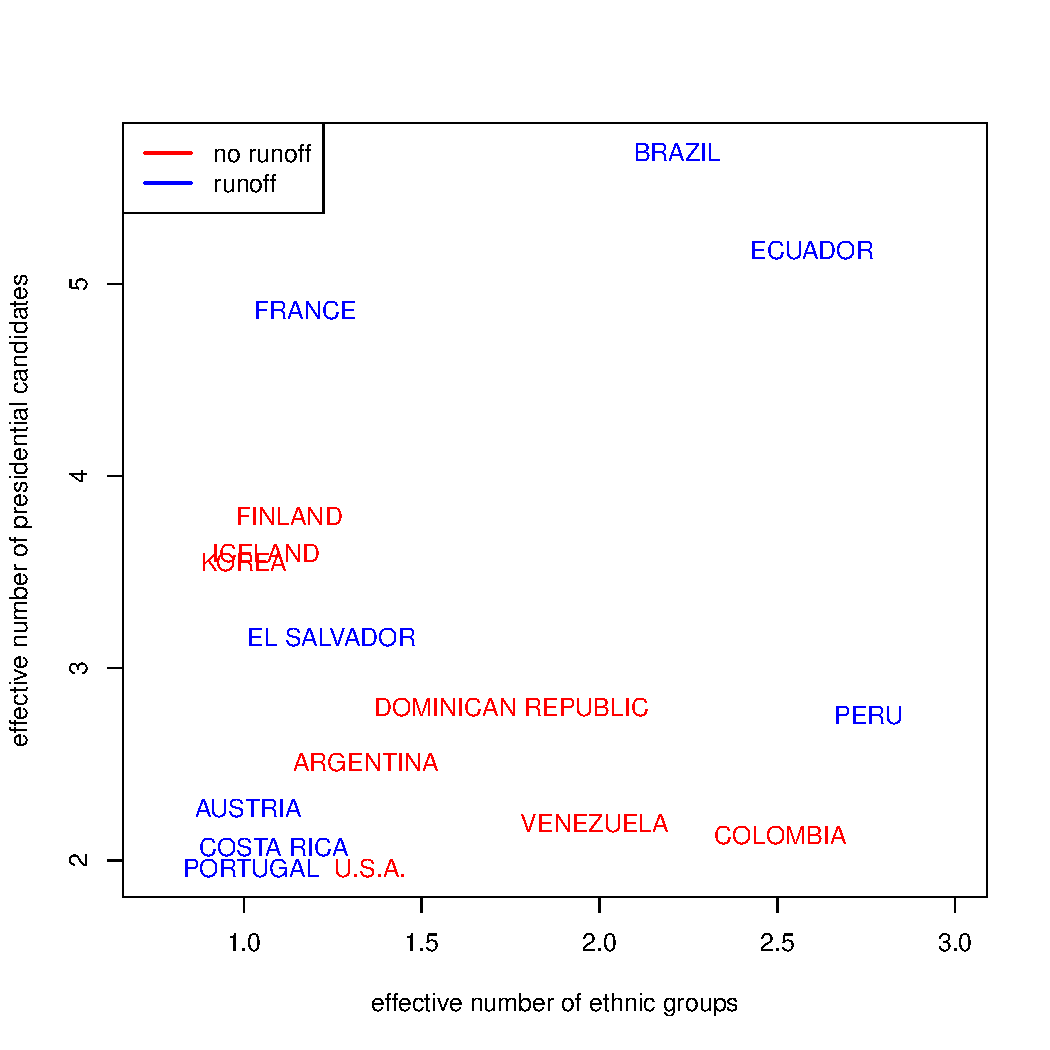
\includegraphics[height=3in]{figures/p1.pdf}
  \end{center}
  \vspace{-0.275in}
\end{figure}

}

\frame{
\frametitle{Additive Linear Regression}

\begin{figure}[ht]
  \begin{center}
    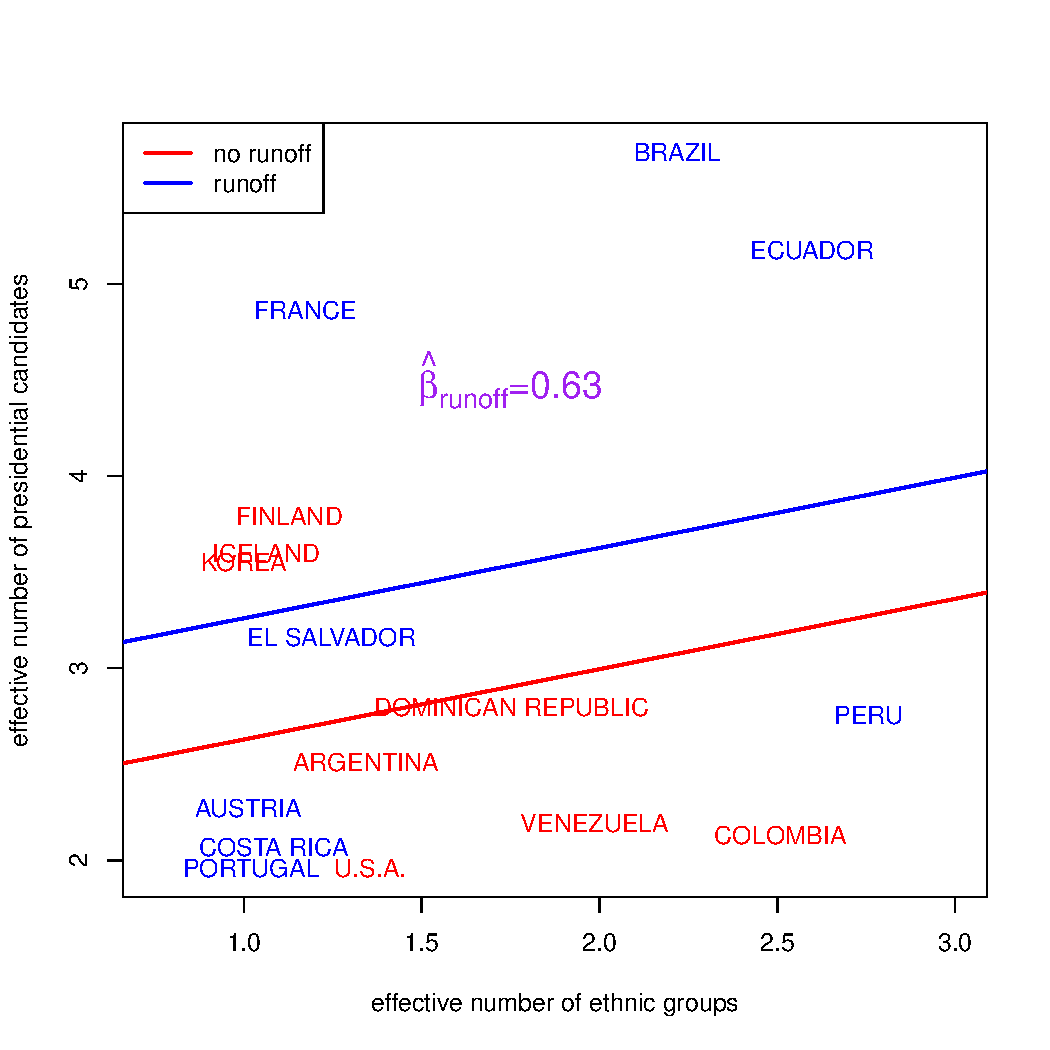
\includegraphics[height=3in]{figures/p2.pdf}
  \end{center}
  \vspace{-0.275in}
\end{figure}

}

\frame{
\frametitle{Average Partial Derivative (Runoff) in Additive Model}

\begin{figure}[ht]
  \begin{center}
    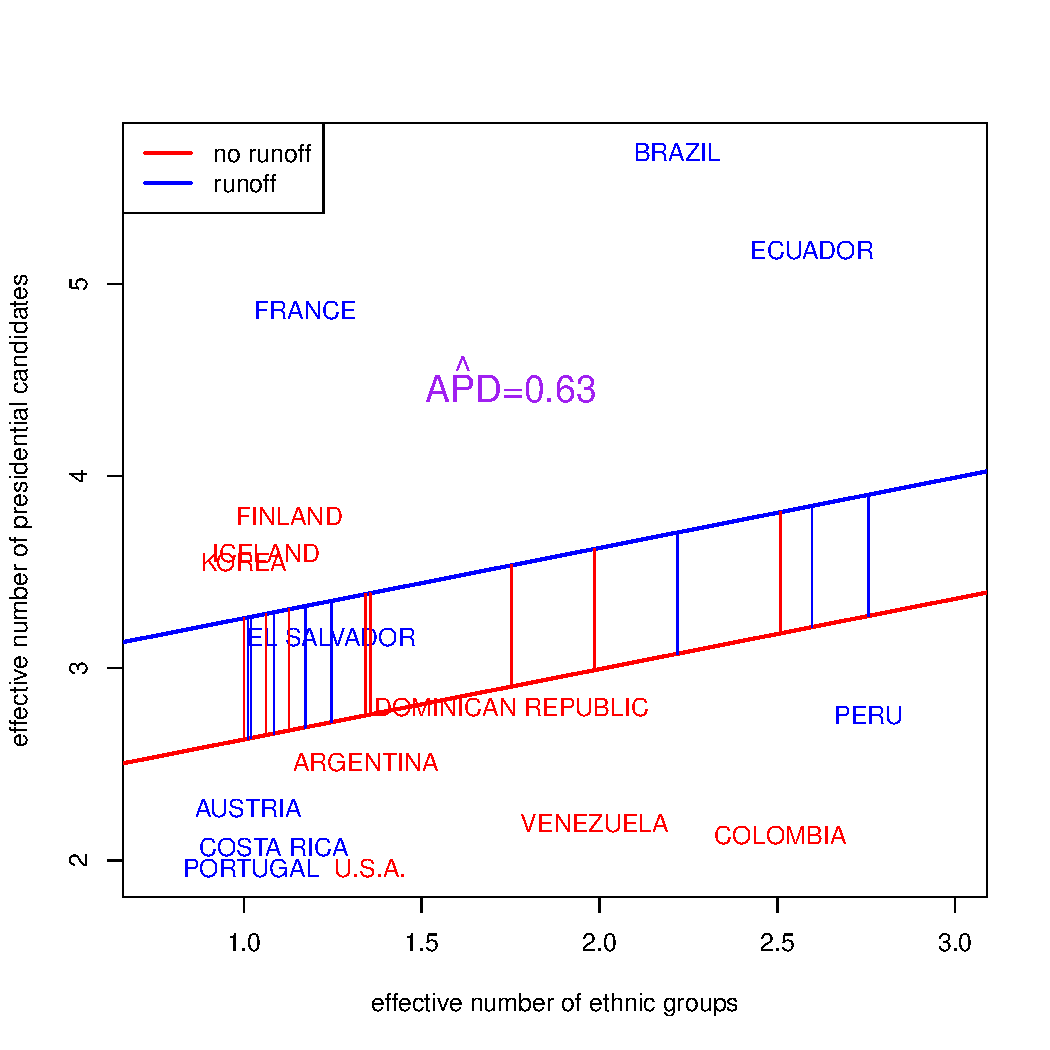
\includegraphics[height=3in]{figures/p2b.pdf}
  \end{center}
  \vspace{-0.275in}
\end{figure}

}

\frame{
\frametitle{APD in Interactive/Unpooled Linear Model}

\begin{figure}[ht]
  \begin{center}
    \includegraphics<1>[height=3in]{figures/p3.pdf}
    \includegraphics<2>[height=3in]{figures/p4b.pdf}
  \end{center}
  \vspace{-0.275in}
\end{figure}

}

\frame{
\frametitle{APD in Additive Quadratic Models}

\begin{figure}[ht]
  \begin{center}
    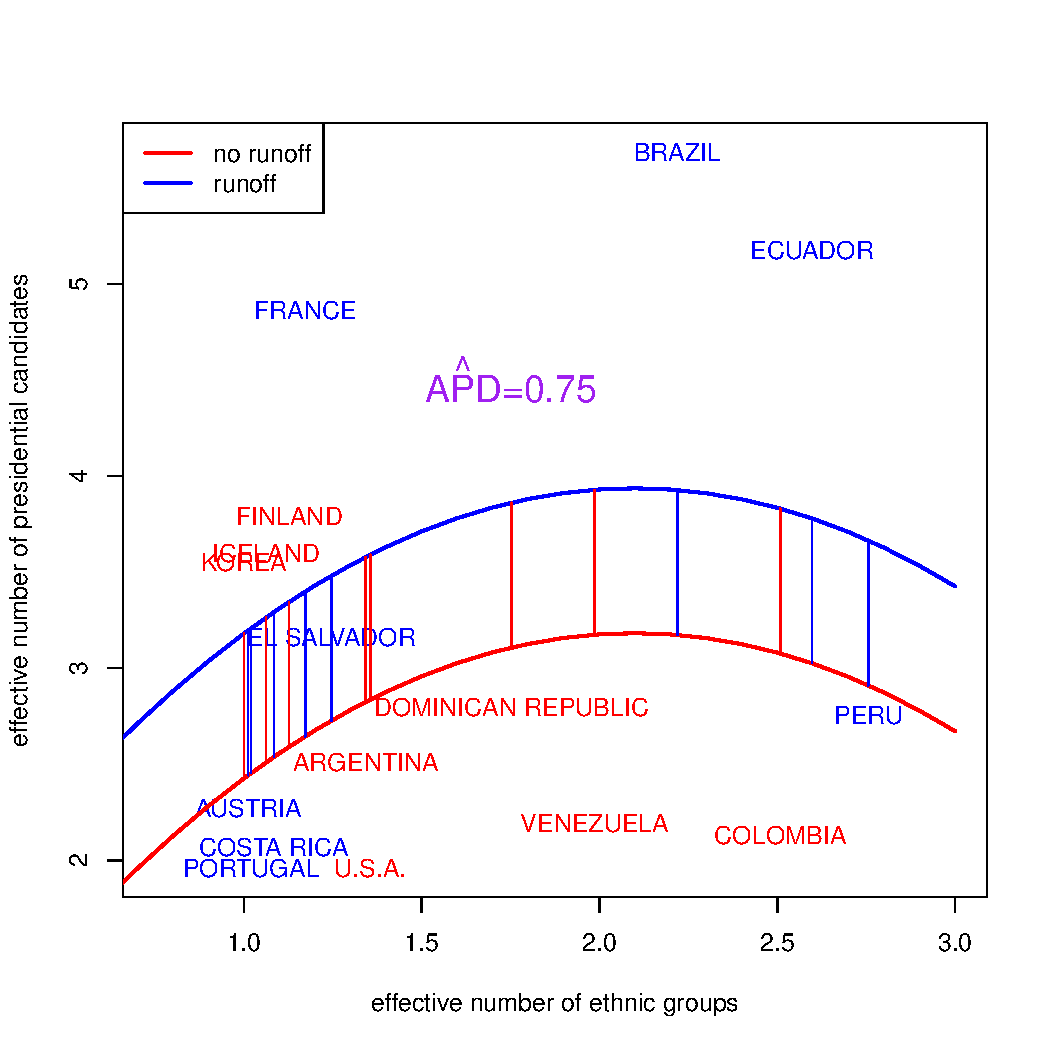
\includegraphics[height=3in]{figures/p13b.pdf}
  \end{center}
  \vspace{-0.275in}
\end{figure}

}


\frame{
\frametitle{APD in Interactive/Unpooled Quadratic}

\begin{figure}[ht]
  \begin{center}
    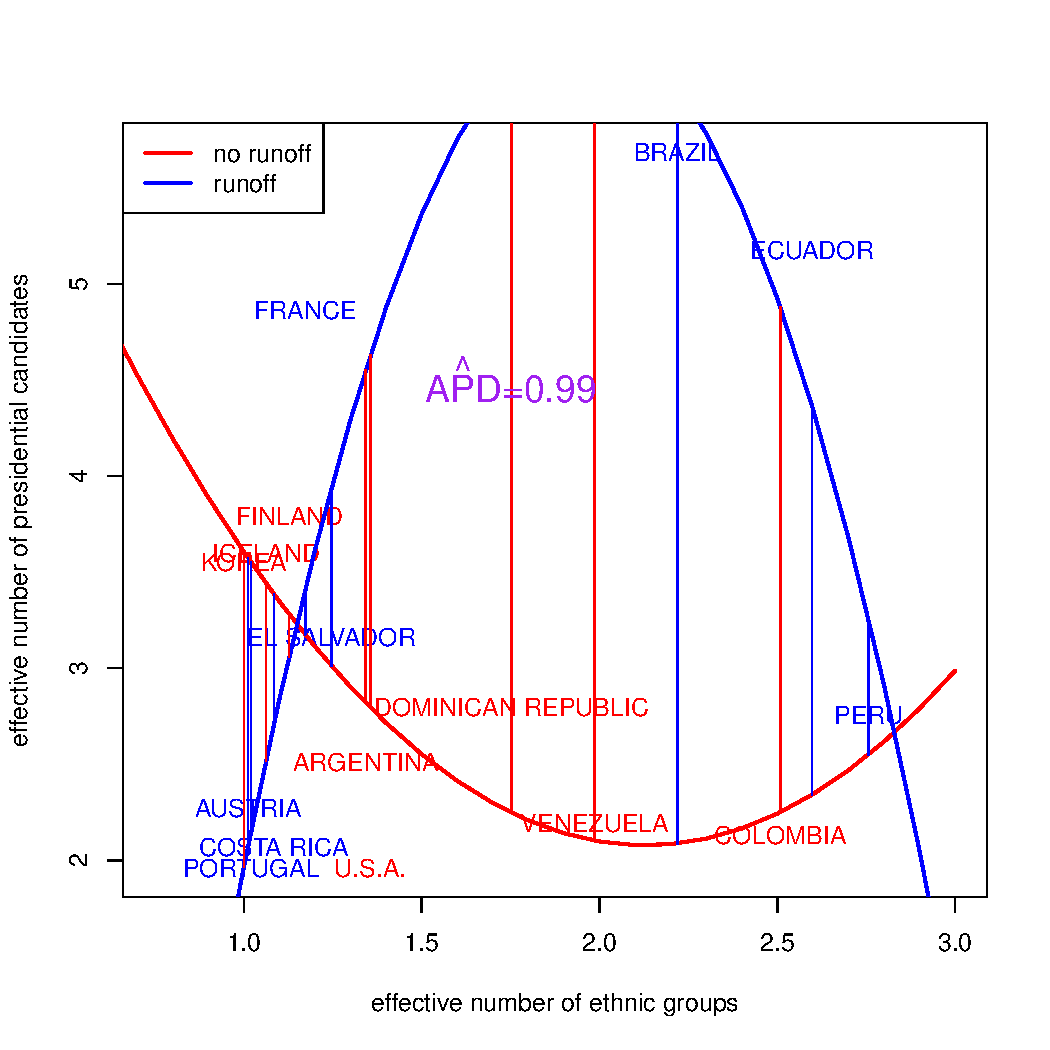
\includegraphics[height=3in]{figures/p13c.pdf}
  \end{center}
  \vspace{-0.275in}
\end{figure}

}

\frame{
\frametitle{APD in Unpooled Local Regression}

\begin{figure}[ht]
  \begin{center}
    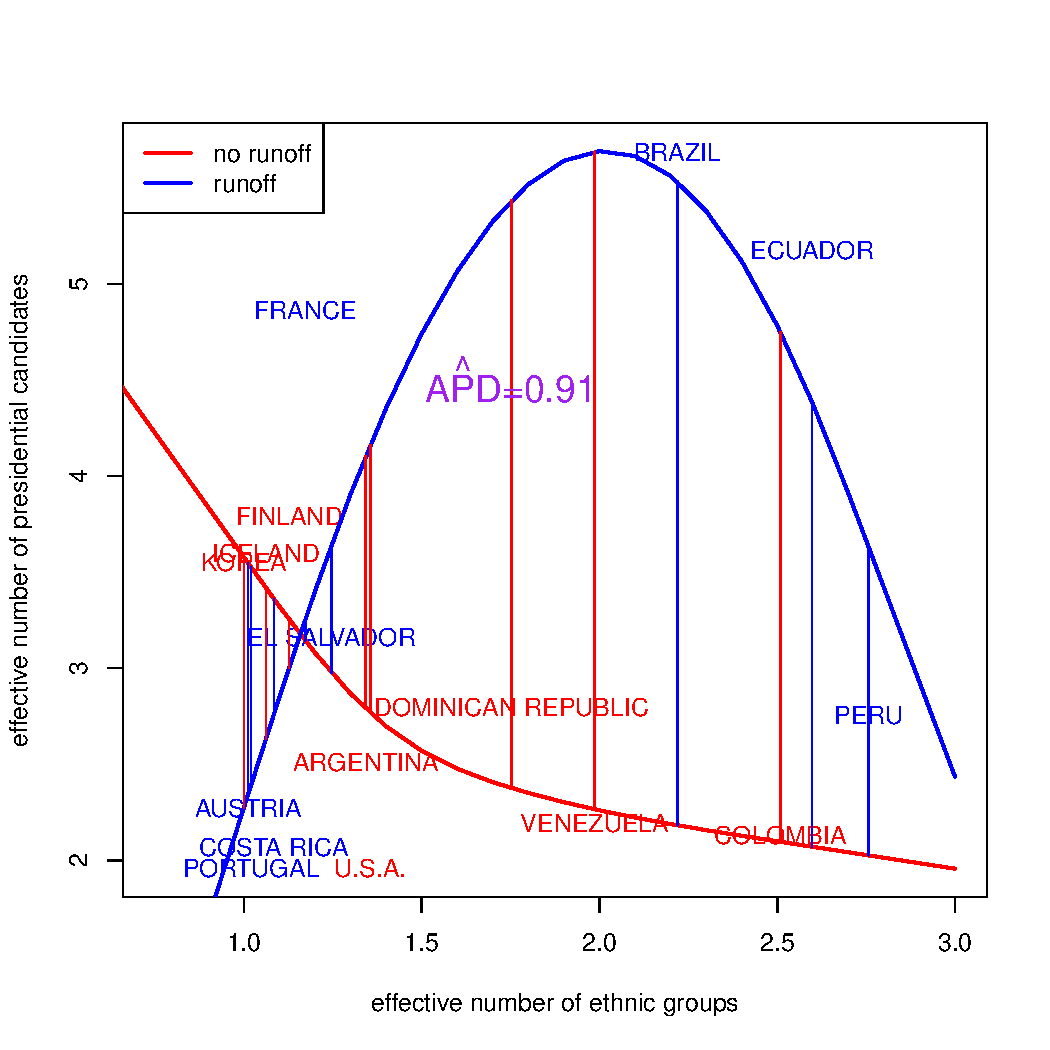
\includegraphics[height=3in]{figures/p15d.pdf}
  \end{center}
  \vspace{-0.275in}
\end{figure}

}




\frame{
\frametitle{APD (Runoff) for the Runoff Countries in Interactive Linear Model}

\begin{figure}[ht]
  \begin{center}
    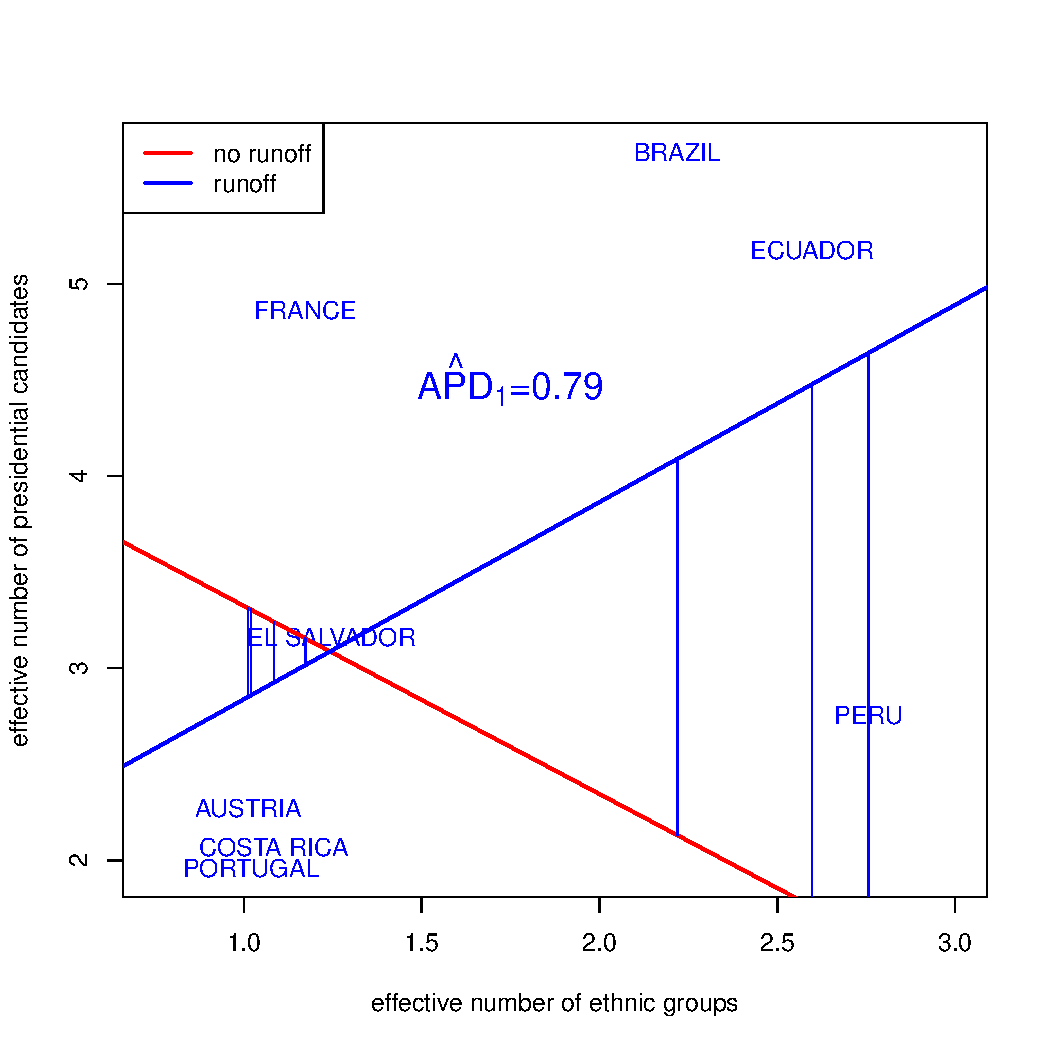
\includegraphics[height=3in]{figures/p5.pdf}
  \end{center}
  \vspace{-0.275in}
\end{figure}

}

\frame{
\frametitle{APD (Runoff) for the Non-Runoff Countries in Interactive Linear Model}

\begin{figure}[ht]
  \begin{center}
    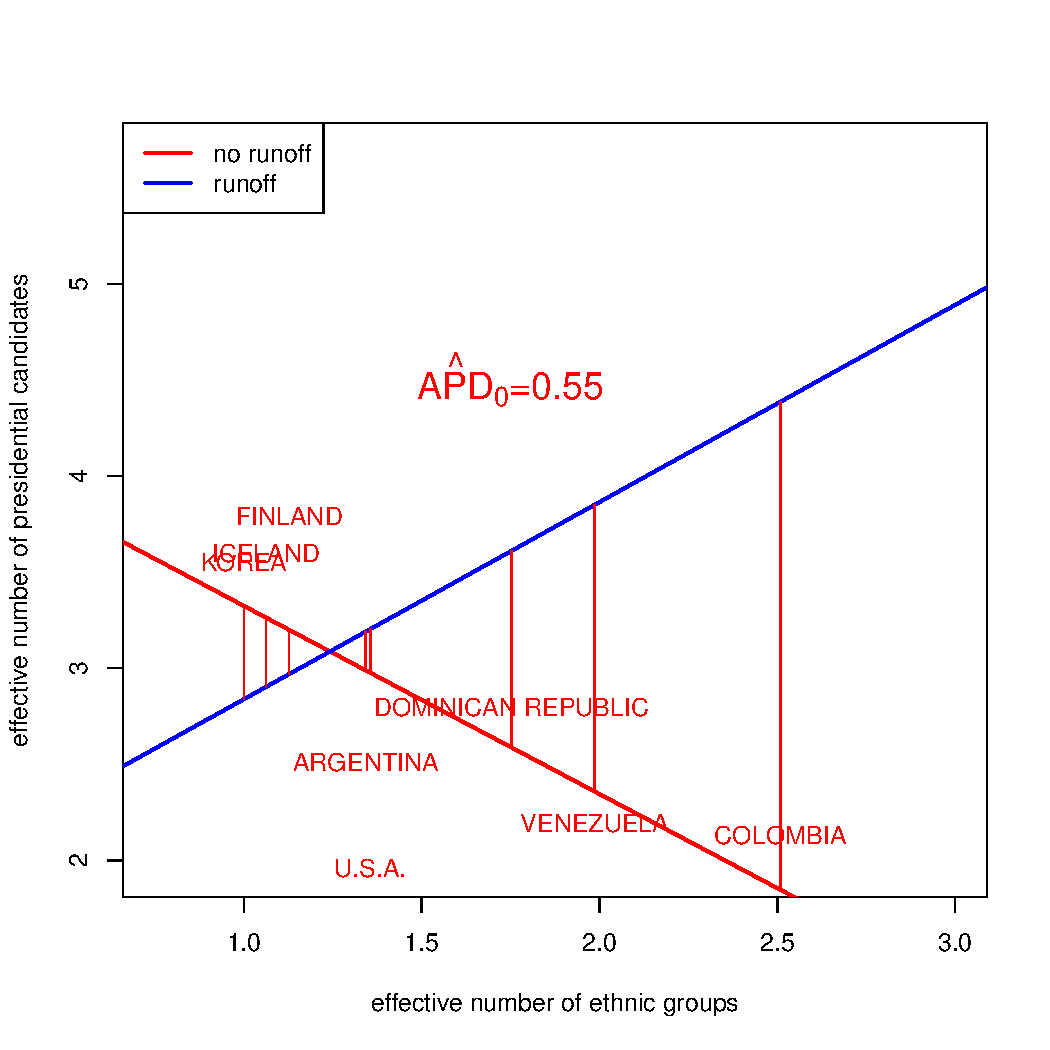
\includegraphics[height=3in]{figures/p6.pdf}
  \end{center}
  \vspace{-0.275in}
\end{figure}

}

\frame{

Mathematical Presentation

}

\frame{

What if the CEF is nonlinear?

\vspace{0.2in}

I.e., what if $\E[Y | X] \neq a + bX$?

\vspace{0.2in}

Can we still use linear regression?

}

%
%
%\frame{
%
%Today, I will detail the bivariate case.
%
%}
%


%\frame{
%
%\begin{center}
%%\includegraphics[width=0.75\textwidth]{nonlin1.PDF}
%
%\end{center}
%}
%
%\frame{
%
%\begin{center}
%%\includegraphics[width=0.75\textwidth]{nonlin2.PDF}
%
%\end{center}
%}
%
%\frame{
%
%The CEF is nonlinear $\E[Y | X] = 10 X^2$. But what would the BLP be?
%
%}
%
%\frame{
%
%\begin{center}
%%\includegraphics[width=0.75\textwidth]{nonlin3.PDF}
%
%\end{center}
%}




\frame{

When the CEF is linear in $X$, $X^2$,

 $$ \E[Y | X] = \beta_0 + \beta_1 X + \beta_2 X^2.$$

}



\frame{
How to interpret?

\vspace{0.2in}

Before: linear estimate of slope of CEF was $\beta_1$.

\vspace{0.2in}

How can we generalize?

}

\frame{

When the CEF is linear in $X$, $X^2$,

$$\frac{\partial \E[Y | X]}{\partial X} = \frac{\partial (\beta_0 +  \beta_1  X + \beta_2 X^2)}{\partial X}$$

}

\frame{

When the CEF is linear in $X$, $X^2$,

$$\frac{\partial \E[Y | X]}{\partial X} = \beta_1 + 2 \beta_2 X$$

}

\frame{

When the CEF is linear in $X$, $X^2$,

$$\frac{\partial \E[Y | X]}{\partial X} = \beta_1 + 2 \beta_2 X$$

\vspace{0.2in}

The slope of the CEF depends on the value of $X$.

}


%
%
%\frame{
%
%\begin{center}
%%\includegraphics[width=0.75\textwidth]{nonlin2.PDF}
%
%\end{center}
%}
%
%%\frame{
%%
%%When the CEF is not linear in $X$, $X^2$,
%%
%%$$\frac{\partial \E[Y | X]}{\partial X} \approx \beta_1 + 2 \beta_2 X$$
%%
%%}
%
%\frame{
%
%Can we develop a general result for approximating the CEF with polynomials?
%
%}
%
%
%\frame{
%
%\begin{center}
%%\includegraphics[width=0.75\textwidth]{poly.PDF}
%\end{center}
%}
%
%\frame{
%
%Let's approximate the CEF with polynomials of $X$.
%
%}
%
%%\frame{
%%
%%\begin{center}
%%\includegraphics[width=0.75\textwidth]{poly1.PDF}
%%\end{center}
%%}
%%\frame{
%%
%%\begin{center}
%%\includegraphics[width=0.75\textwidth]{poly2.PDF}
%%\end{center}
%%}
%%\frame{
%%
%%\begin{center}
%%\includegraphics[width=0.75\textwidth]{poly3.PDF}
%%\end{center}
%%}
%%\frame{
%%
%%\begin{center}
%%\includegraphics[width=0.75\textwidth]{poly4.PDF}
%%\end{center}
%%}
%%\frame{
%%
%%\begin{center}
%%\includegraphics[width=0.75\textwidth]{poly5.PDF}
%%\end{center}
%%}
%%
%%\frame{
%%
%%\begin{center}
%%\includegraphics[width=0.75\textwidth]{poly10.PDF}
%%\end{center}
%%}
%
%\frame{
%
%I am not saying that it is good practice to include a polynomial of length 10!
%
%\vspace{0.2in}
%
%But the point holds. We can always approximate the CEF to arbitrary precision, as long as it's continuous -- even when it's not smooth [i.e., differentiable]!
%
%}
%
%\frame{
%
%When we think about regression as a way to estimate expected values, we see that linearity doesn't matter -- it can be arbitrarily relaxed.
%
%}
%
%
%\frame{
%
%To formalize a bit. Suppose $\E[Y | x]$ is continuous and $\Supp(X) = [a,b]$, then for any positive $\epsilon$ and for all integers $K' \geq K$, there always exists a $K$ such that:
%$$
%\E\left[ \left(\E[Y | x] - \left(\beta_0 + \beta_1 x + \beta_2 x^2 + ... + \beta_{K'} x^{K'}\right)\right)^2\right] < \epsilon,
%$$
%where the $\beta_k$s denote the BLP coefficients with respect to $(1,X,X^2,...,X^{K'})$ . Proof follows from Weierstrass and MMSE properties of the BLP.
%
%}

%\frame{
%
%To formalize a bit. Suppose $\E[Y | x]$ is continuous and $\Supp(X) = [a,b]$, then for any positive $\epsilon$ and for all integers $K' \geq K$, there always exists a $K$ such that:
%$$
%\E\left[ \left(\E[Y | x] - \sum_{k=0}^{K} \beta_k\right)^2\right] < \epsilon,
%$$
%where the $\beta_k$s denote the BLP coefficients with respect to $(1,X,X^2,...,X^{K'})$ . Proof follows from Weierstrass and MMSE properties of the BLP.
%
%}
%
%
%%\frame{
%%
%%To formalize a bit. For continuous $\E[Y | x]$, then for any positive $\epsilon$, there always exists a $K$, such that:
%%$$
%%\E[ \E[Y | x] - \left(\beta_0 + \beta_1 x + \beta_2 x^2 + ... + \beta_K x^K\right))^2] < \epsilon,
%%$$for all values of $x \in [a,b]$.
%%
%%}
%
%\frame{
%
%So as long as you're willing to be sufficiently flexible in how you write out your regressors, you can always do a pretty good job approximating the CEF.
%
%\vspace{0.2in}
%
%So if you're worried about the linearity in linear regression, you can relax it without much issue. Polynomials are just one way [high-order polynomials are not a particularly good way, for rather complicated reasons]. In the next class, I will detail others.
%
%}
%
%\frame{
%
%Example from book.
%
%}

%\frame{
%
%See overfitting example from book, but what about a more formal criteria.
%
%}
%
%\frame{
%\frametitle{Bias/Var Tradeoff}
%
%Recall the estimators:
%\begin{align*}
%\overline{Y^2} -&  \overline{Y}^2 \\
%\frac{n}{n-1}[\overline{Y^2} -&  \overline{Y}^2]
%\end{align*}
%
%Compare the two on bias and variance.
%
%}
%
%\frame{
%
%Go to regression bias/variance tradeoff example
%
%}


\frame{

What about multiple $X$:
\begin{itemize}
\item Additive, Interactive, and Saturated Models
\item with polynomials
\item What if not linear in $\beta$?
%\item statistical/machine learning approaches
\end{itemize}

}


%
%\frame{
%
%[Looking at data.]
%
%}
%
%\frame{
%
%Next class: discrete regressors, interaction terms, saturated models.
%
%}
%
%
%\frame{
%
%Nonlinearity in the CEF, part II.
%
%\vspace{0.2in}
%
%(Or: if you can't find a way to do it with linear regression, you probably shouldn't be doing it.)
%
%}
%
%\frame{
%
%How we'll proceed today:
%\begin{itemize}
%\item Interactions between variables
%\item Binary regressors
%\item Saturated models
%\item Real example: QOG data
%\end{itemize}
%
%}
%
%\frame{
%
%Last class, I showed that, with polynomials, we could arbitrarily approximate any sort of nonlinearity in CEF in one variable.
%
%\vspace{0.2in}
%
%In many ways, this was a proof of concept. This principle generalizes to the multivariate case.
%
%}
%
\frame{

What happens when the conditional slope of the CEF with respect to $X_1$ depends on the value of $X_2$?

\vspace{0.2in}

The BLP is still the BLP, but we might be missing out on an interesting {\it interaction} between the variables $X_1$ and $X_2$.

}

\frame{

So, to formalize a bit, what if the CEF is otherwise linear, but includes an {\it interaction}?
$$
\E[Y  | X_1, X_2] = \beta_0 + \beta_1 X_1 + \beta_2 X_2 + \beta_3 X_1 X_2
$$

}


\frame{

Much as before, we could derive the slope of the CEF with respect to a given variable.
$$
\frac{\partial \E[Y  | X_1, X_2]}{\partial X_1} = \frac{\partial \beta_0 + \beta_1 X_1 + \beta_2 X_2 + \beta_3 X_1 X_2}{\partial X_1}.
$$

}


\frame{

Much as before, we could derive the slope of the CEF with respect to a given variable.
$$
\frac{\partial \E[Y  | X_1, X_2]}{\partial X_1} = \beta_1 + \beta_3 X_2.
$$

}


\frame{

$$
\frac{\partial \E[Y  | X_1, X_2]}{\partial X_1} = \beta_1 + \beta_3 X_2.
$$

The conditional slope of the CEF with respect to $X_1$ {\it depends on the value} of $X_2$.

}





%%
%%\frame{
%%
%%$$
%%\frac{\partial \E[Y  | X_1, X_2]}{\partial X_1} = \beta_1 + \beta_3 X_2.
%%$$
%%
%%The conditional slope of the CEF with respect to $X_1$ {\it depends on the value} of $X_2$.
%%
%%}
%
%\frame{
%
%How to read the coefficients then? If the CEF is linear in $X_1$, $X_2$ and $X_1 X_2$,
%
%$$
%\E[Y  | X_1, X_2] = \beta_0 + \beta_1 X_1 + \beta_2 X_2 + \beta_3 X_1 X_2
%$$
%
%\begin{itemize}
%\item $\beta_0$ is the value of $\E[Y  | X_1 = 0, X_2=0]$.
%\item $\beta_1$ is the slope of the CEF w.r.t. $X_1$ when $X_2 = 0$.
%\item $\beta_2$ is the slope of the CEF w.r.t. $X_2$ when $X_1 = 0$.
%\item $\beta_3$ is how each of the slopes changes, when you move one unit in the other variable
%\begin{itemize}
%\item I.e., if $X_2$ moves from $0$ to $1$, then the slope of the CEF w.r.t. $X_1$ changes by $\beta_3$.
%\item I.e., if $X_1$ moves from $4$ to $7$, then the slope of the CEF w.r.t. $X_2$ changes by $3 \beta_3$.
%\end{itemize}
%\end{itemize}
%
%}
%
%\frame{
%
%How to read the coefficients then? If the CEF is linear in $X_1$, $X_2$ and $X_1 X_2$,
%
%$$
%\E[Y  | X_1, X_2] = \beta_0 + \beta_1 X_1 + \beta_2 X_2 + \beta_3 X_1 X_2
%$$
%
%\vspace{0.2in}
%
%If $\beta_3 = 0$, then $\E[Y  | X_1, X_2] = \beta_0 + \beta_1 X_1 + \beta_2 X_2$, and the interaction is irrelevant.
%
%}
%
\frame{

For full generality, interactions can be combined with polynomials, e.g.:
$$
\E[Y  | X_1, X_2] = \beta_0 + \beta_1 X_1 + \beta_2 X_2 + \beta_3 X_1 X_2 + \beta_4 X_2^2 + \beta_5 X_1^2 X_2
$$

With slopes computed by taking partial derivatives.

\bigskip

Let's find

$$
\frac{\partial \E[Y|\X]}{\partial X_1}|_{\X=x}
$$


}
%
%\frame{
%
%In general, what's the easiest way to interpret?
%
%\vspace{0.2in}
%
%Just compute the implied $\E[Y | X_1, X_2]$ for different values of $X_1$, $X_2$. You can always interpret the coefficients straightforwardly.
%
%}
%
%\frame{
%
%Again, linear regression (OLS) yields a consistent estimate of the $\beta$s for any of the above specifications.
%
%\vspace{0.2in}
%
%Recall: when the CEF is not linear in the defined variables, you're just estimating the features of the BLP. I.e., it's a good principled guess of the CEF.
%
%}
%
%%\frame{
%%
%%Remember: the CEF characterizes the expected value of $Y$ given certain values of $X_1$ and $X_2$.
%%
%%\vspace{0.2in}
%%
%%The ``regular" BLP approximates the CEF, in part, but ruling out the idea that conditional slopes depend on
%%
%%}
%
%
%%
%%\frame{
%%
%%Remember when we derived the expected value, $\E[Y]$, as the MMSE approximation to the unconditional distribution of $Y$?
%%
%%}
%
%
%\frame{
%
%So don't worry about nonlinearity for linear regression.
%\begin{itemize}
%\item It ``usually" doesn't matter all that much for our substantive interpretation.
%\item It can always be relaxed arbitrarily.
%\end{itemize}
%
%}
%
%\frame{
%
%I'm going to discuss a couple more points to reinforce these ideas.
%
%}
%

\frame{
\frametitle{Average Partial Derivative}

The partial derivative can differ for all possible $\X=x$
$$
\frac{\partial \E[Y|\X]}{\partial X_1}|_{\X=x}
$$

Often, we will be interested in an average of these partials

$$
APD_{X_1} = E\left[ \frac{\partial \E[Y|\X]}{\partial X_1}|_{\X=x} \right]
$$
 
where the average is taken over the distribution of $\X$.

}

\frame{
\frametitle{Estimated Average Partial Derivative}

In practice, we just average over the partials at the data points
$$
\widehat{APD}_{X_1} = \frac{1}{n}\sum_{i=1}^n\left[ \frac{\partial \E[Y|\X]}{\partial X_1}|_{\X=x} \right]
$$

}

\frame{
Estimated APD Examples on board:

\bigskip

Single $X$ examples
\bi
\item Linear
\item Quadratic
\item Cubic
\ei

\bigskip

$X_1$,$X_2$ examples
\bi
\item Linear Additive
\item Linear Interactive
\item Polynomial with Interactions
\ei

}




\frame{


Recall the estimated APD:

$$
\widehat{APD}_{X_1} = \frac{1}{n}\sum_{i=1}^n\left[ \frac{\partial \hat \E[Y|\X]}{\partial X_1}|_{\X=x} \right]
$$

What if we had a binary regressor, $X_1$ (i.e., $\Supp(X_1) = \{0,1\}$)? \pause

\small

\begin{align*}
\widehat{APD}_{X_1} &= \frac{1}{n}\sum_{i=1}^n\left[ \hat \E[Y|X_1 = 1,\X_{(-1)}=\x_{i,(-1)}] -   \hat \E[Y|X_1 = 0,\X_{(-1)}=\x_{i,(-1)}] \right]  \\ 
%&= \frac{1}{n}\sum_{i=1}^n\left[ \hat \E[Y|X_1 = 1,\X_{(-1)}=\x_{i,(-1)} ] \right] \\
%&- \frac{1}{n}\sum_{i=1}^n\left[ \hat \E[Y|X_1 = 0,\X_{(-1)}=\x_{i,(-1)} ]\right]
\end{align*}

Note that this is exactly what we did with the Neto and Cox (1997) example!

}


\frame{
\frametitle{Confidence Intervals for APDs}


Just Bootstrap!

}

%\frame{
%\frametitle{Imputation APD for  Non-Runoff Countries}
%
%\begin{figure}[ht]
%  \begin{center}
%    \includegraphics<1>[height=3in]{figures/p7.pdf}
%    \includegraphics<2>[height=3in]{figures/p8.pdf}
%    \includegraphics<3>[height=3in]{figures/p8b.pdf}
%  \end{center}
%  \vspace{-0.275in}
%\end{figure}
%
%}
%
%\frame{
%\frametitle{Imputation APD for  Non-Runoff Countries}
%
%\begin{figure}[ht]
%  \begin{center}
%    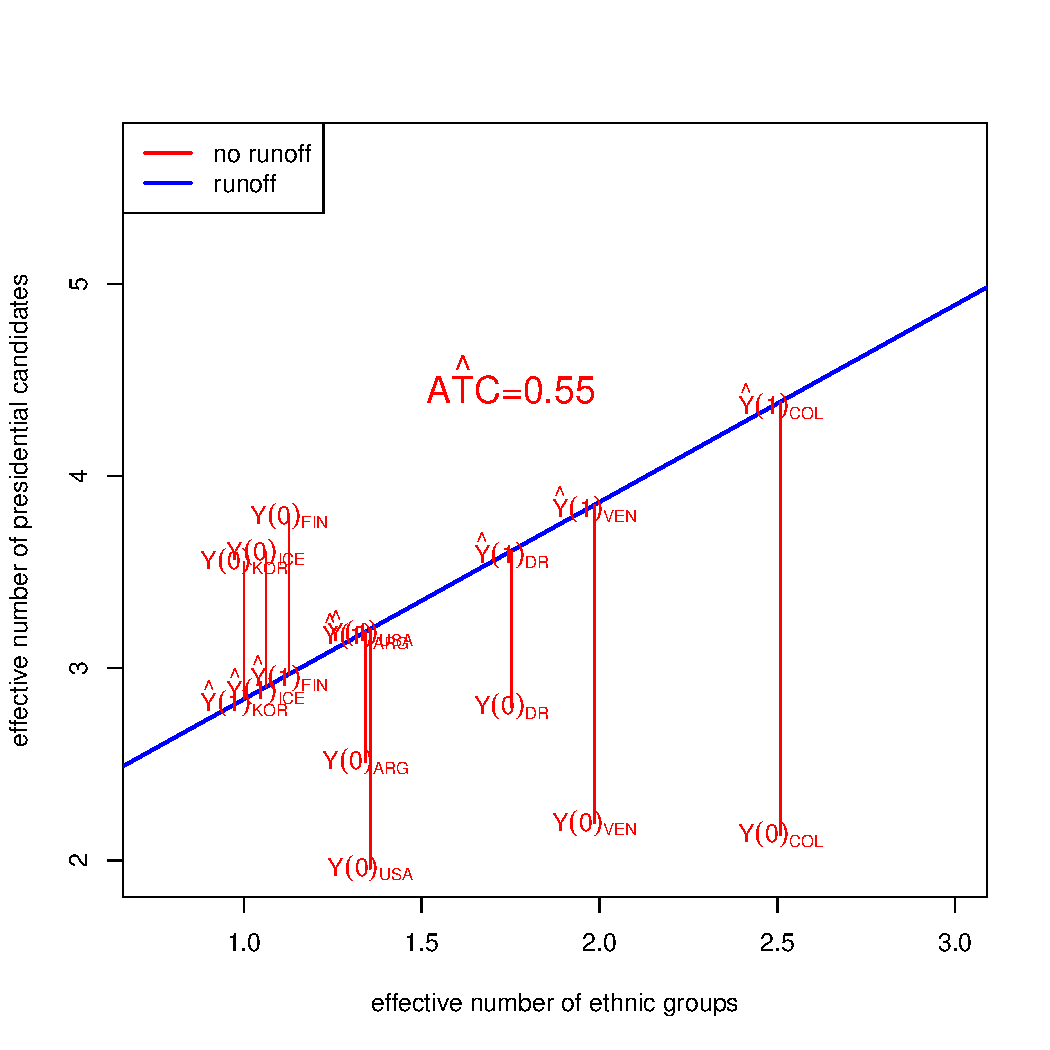
\includegraphics[height=3in]{figures/p9.pdf}
%  \end{center}
%  \vspace{-0.275in}
%\end{figure}
%
%}

%\frame{
%\frametitle{Diagnostics}
%
%\begin{figure}[ht]
%  \begin{center}
%    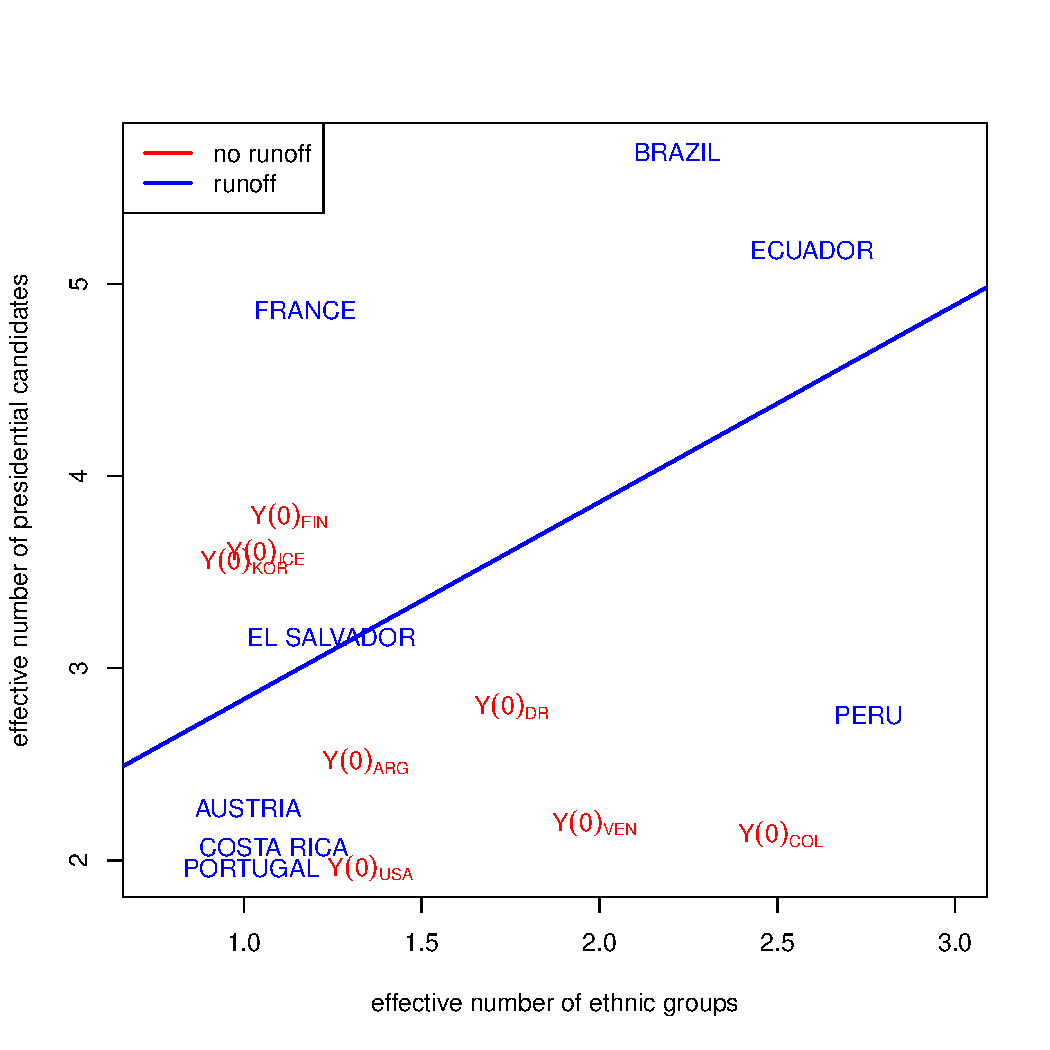
\includegraphics[height=3in]{figures/p10.pdf}
%  \end{center}
%  \vspace{-0.275in}
%\end{figure}
%
%}
%
%\frame{
%\frametitle{Balance and Overlap}
%
%\begin{figure}[ht]
%  \begin{center}
%    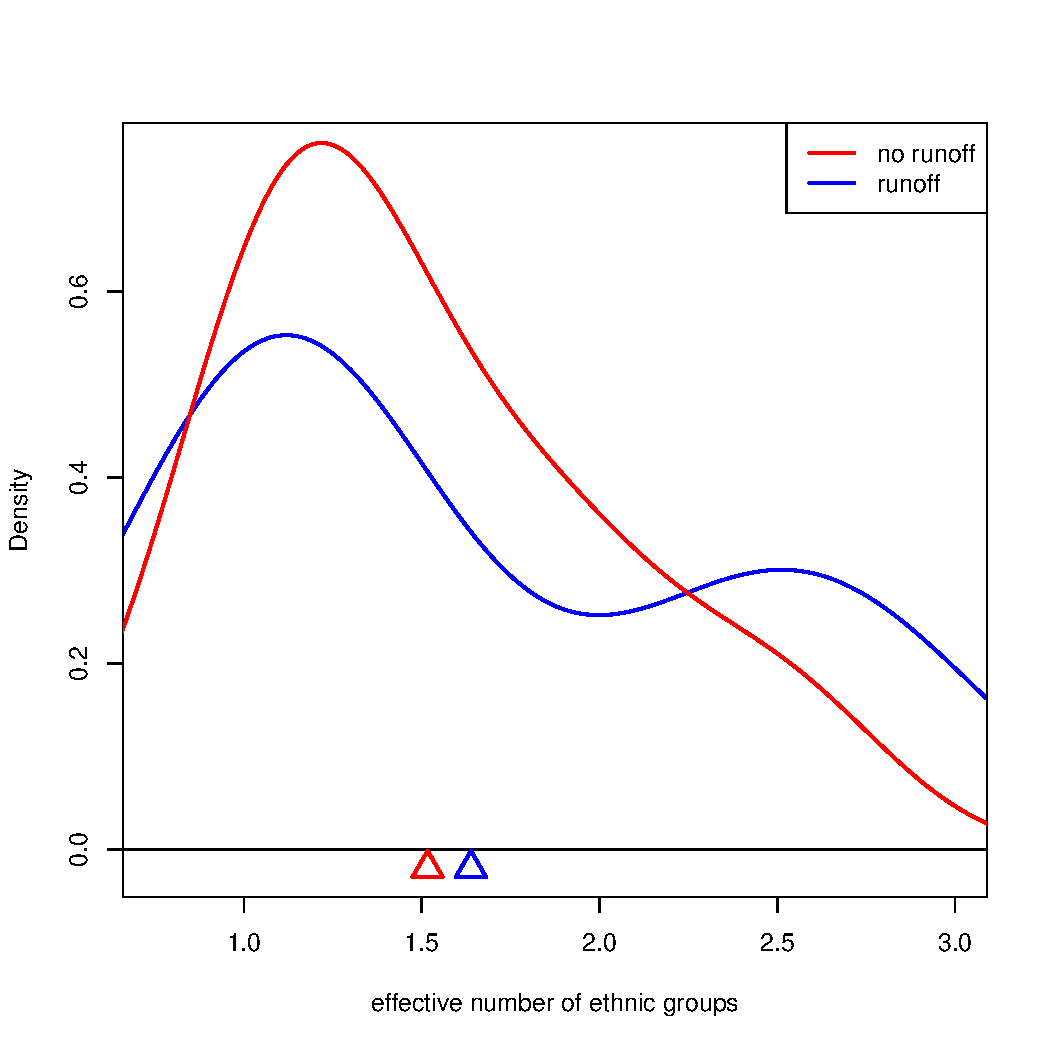
\includegraphics[height=3in]{figures/p11.pdf}
%  \end{center}
%  \vspace{-0.275in}
%\end{figure}
%
%}

%\frame{
%\frametitle{Nonlinearity (Quadratic)}
%
%\begin{figure}[ht]
%  \begin{center}
%    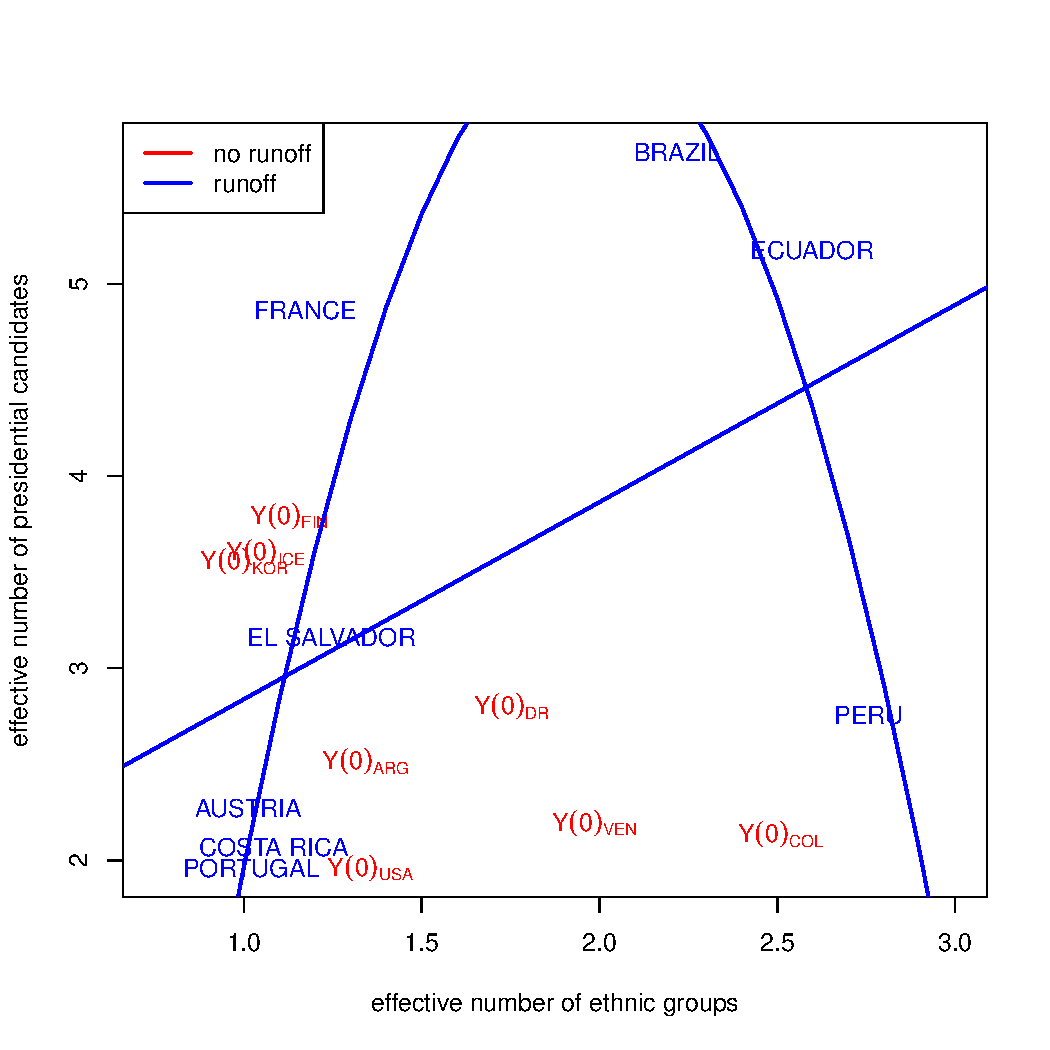
\includegraphics[height=3in]{figures/p12.pdf}
%  \end{center}
%  \vspace{-0.275in}
%\end{figure}
%
%}
%
%\frame{
%\frametitle{APD for Non-runoff Countries with Nonlinearity (Quadratic)}
%
%\begin{figure}[ht]
%  \begin{center}
%    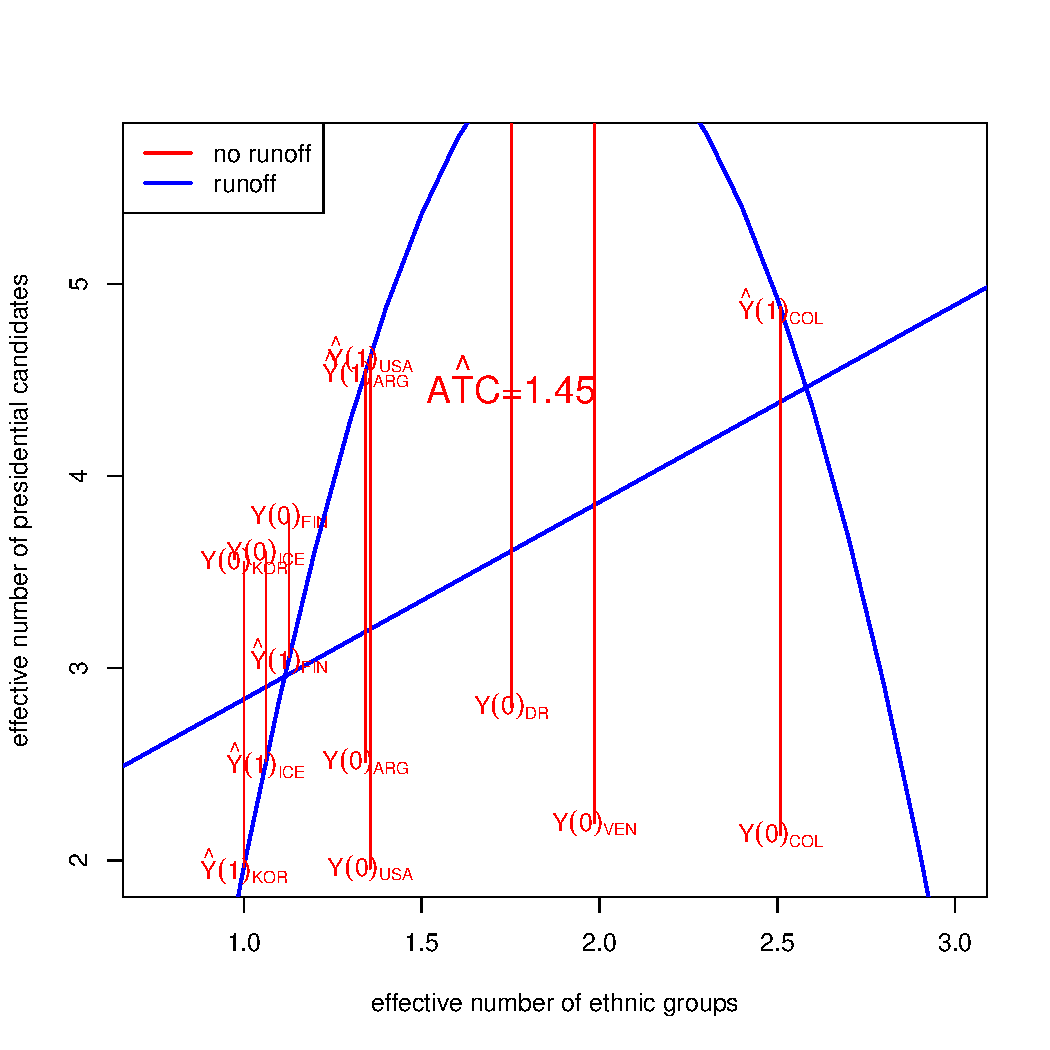
\includegraphics[height=3in]{figures/p13.pdf}
%  \end{center}
%  \vspace{-0.275in}
%\end{figure}
%
%}
%
%\frame{
%\frametitle{APD for Runoff Countries}
%
%\begin{figure}[ht]
%  \begin{center}
%    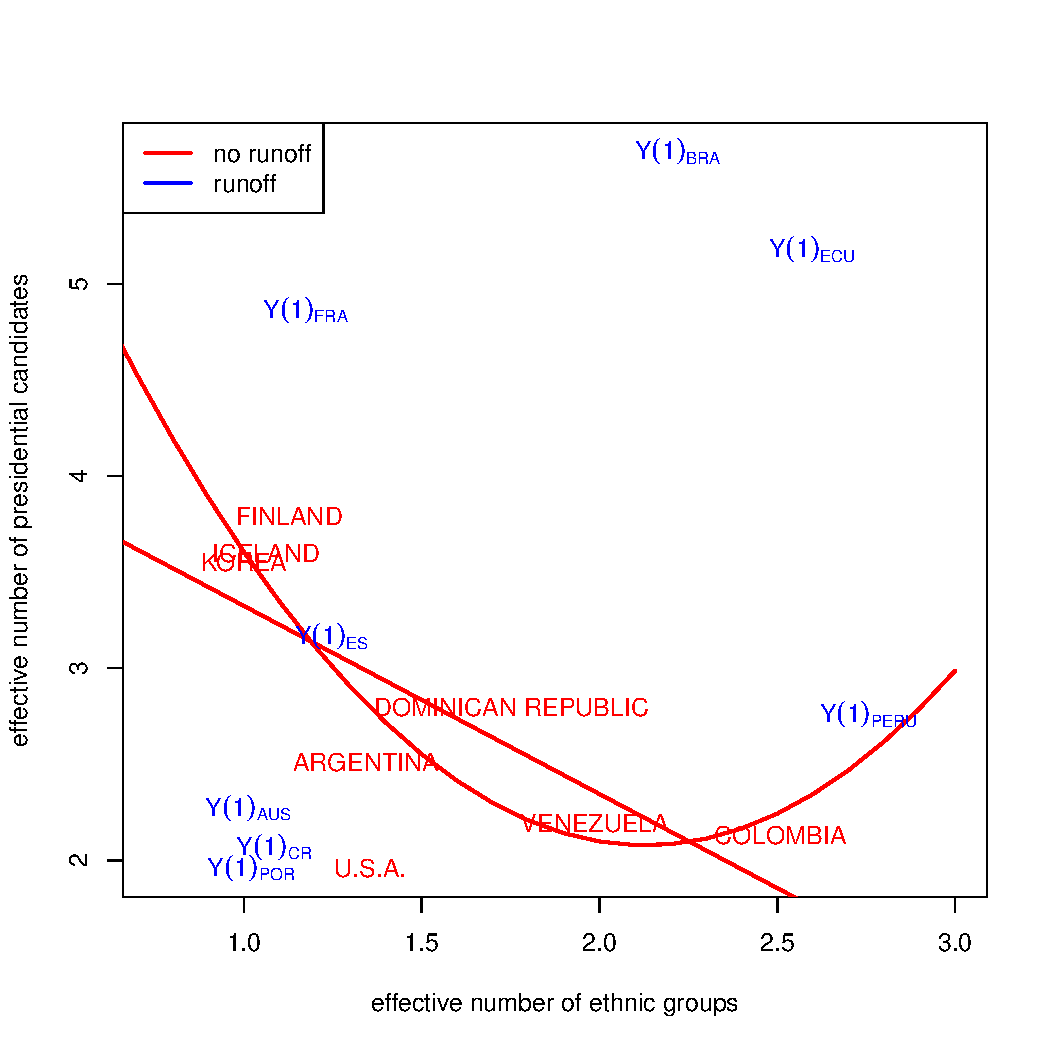
\includegraphics[height=3in]{figures/p14.pdf}
%  \end{center}
%  \vspace{-0.275in}
%\end{figure}
%
%}
%
%
%\frame{
%\frametitle{APD for Runoff Countries (Quadratic)}
%
%\begin{figure}[ht]
%  \begin{center}
%    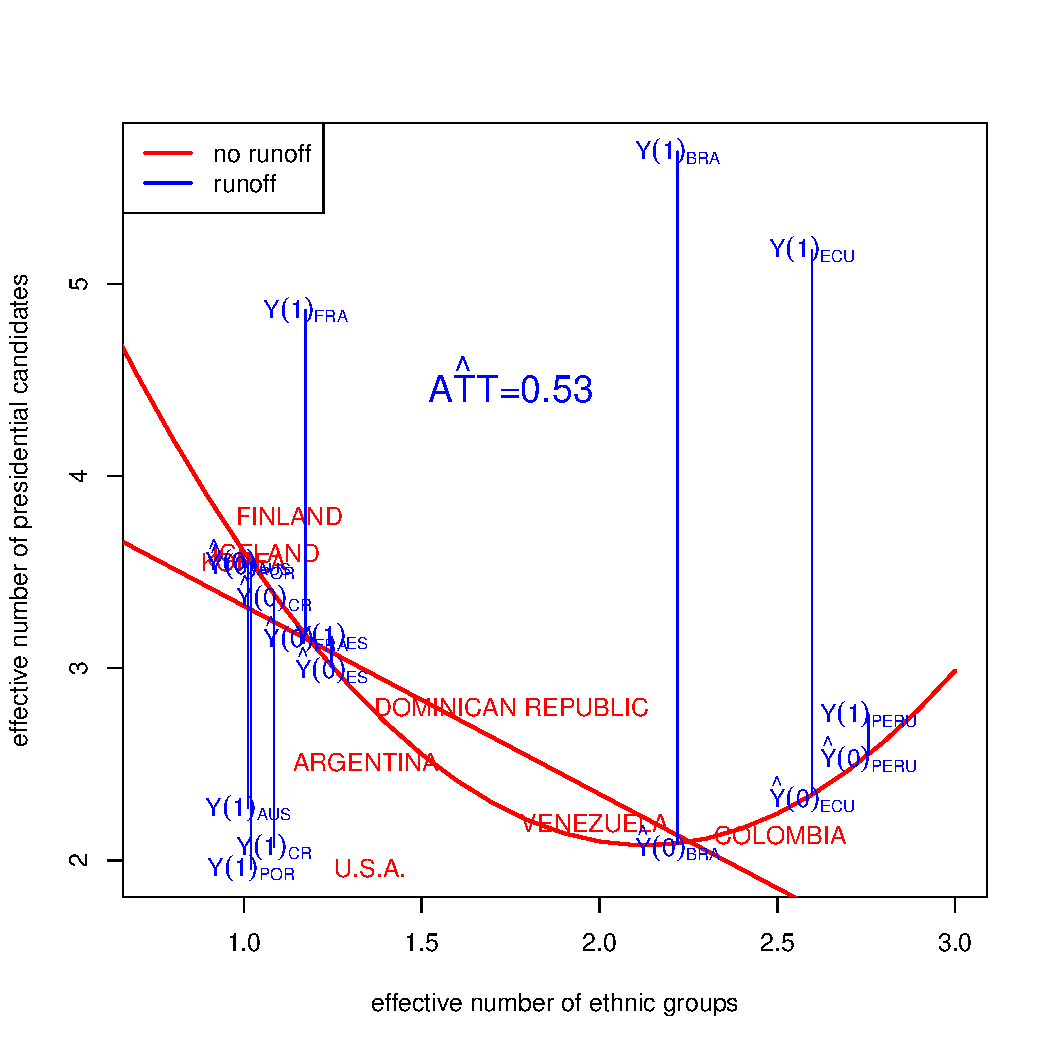
\includegraphics[height=3in]{figures/p15.pdf}
%  \end{center}
%  \vspace{-0.275in}
%\end{figure}
%
%}
%
%\frame{
%\frametitle{APD for Runoff Countries with Local Regression}
%
%\begin{figure}[ht]
%  \begin{center}
%    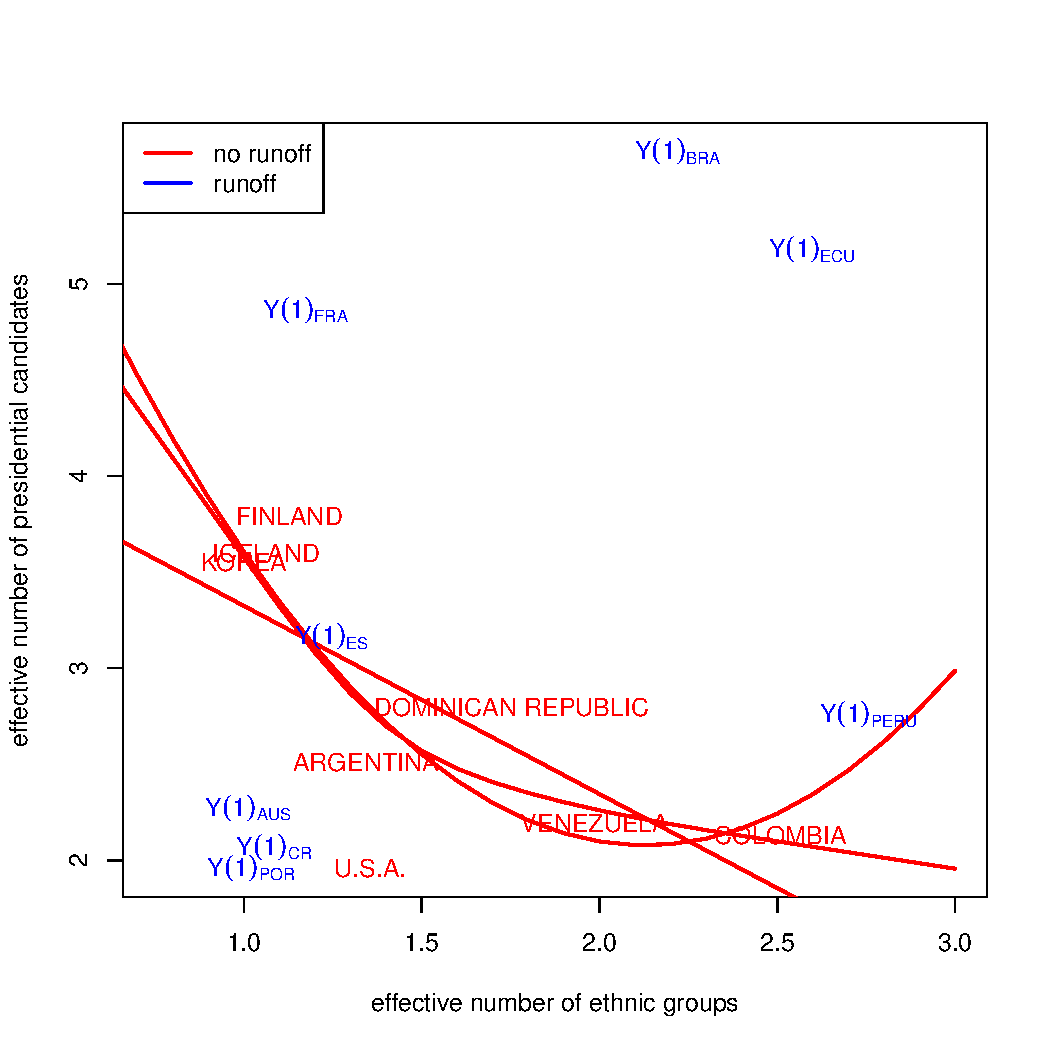
\includegraphics[height=3in]{figures/p15a.pdf}
%  \end{center}
%  \vspace{-0.275in}
%\end{figure}
%
%}
%
%
%\frame{
%\frametitle{APD for Runoff Countries with Local Regression}
%
%\begin{figure}[ht]
%  \begin{center}
%    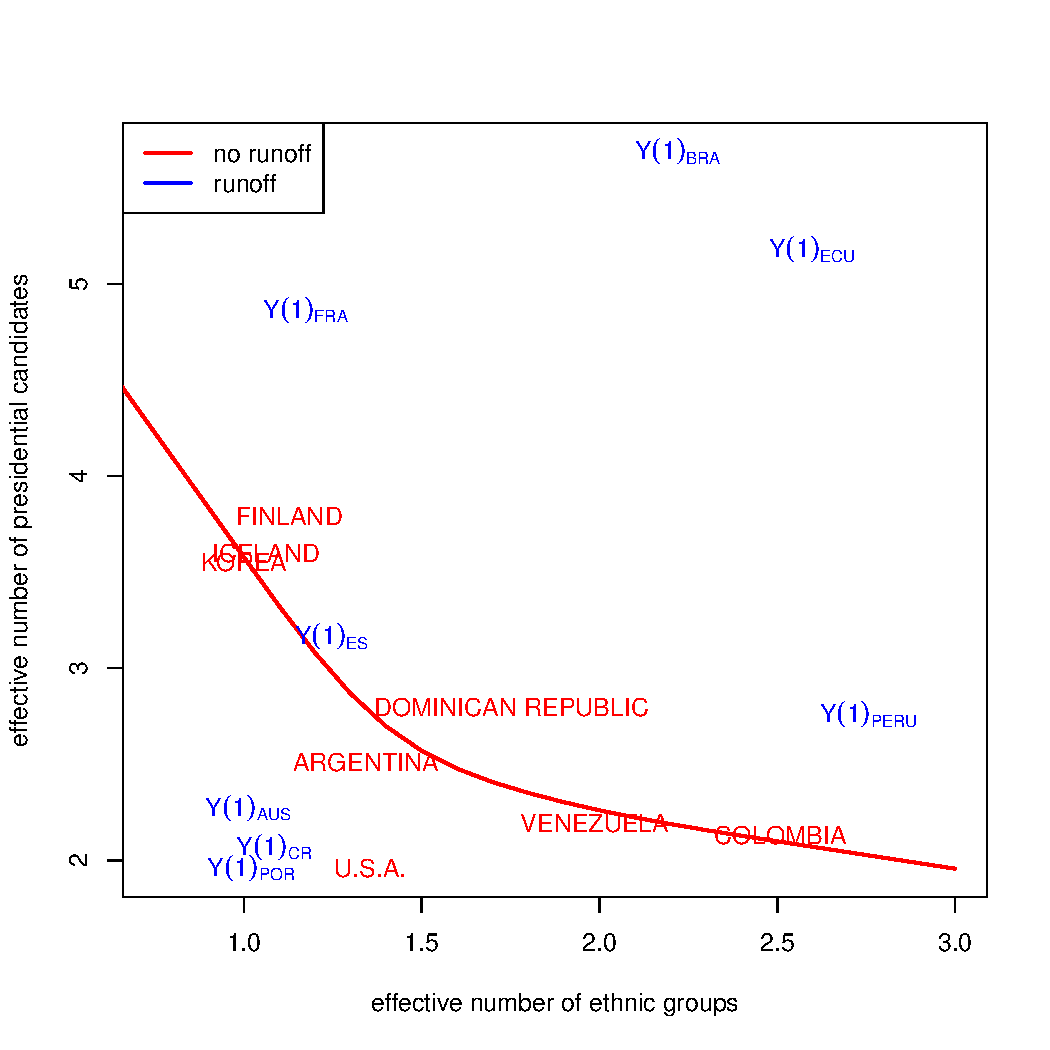
\includegraphics[height=3in]{figures/p15b.pdf}
%  \end{center}
%  \vspace{-0.275in}
%\end{figure}
%
%}
%
%
%\frame{
%\frametitle{APD for Runoff Countries with Local Regression}
%
%\begin{figure}[ht]
%  \begin{center}
%    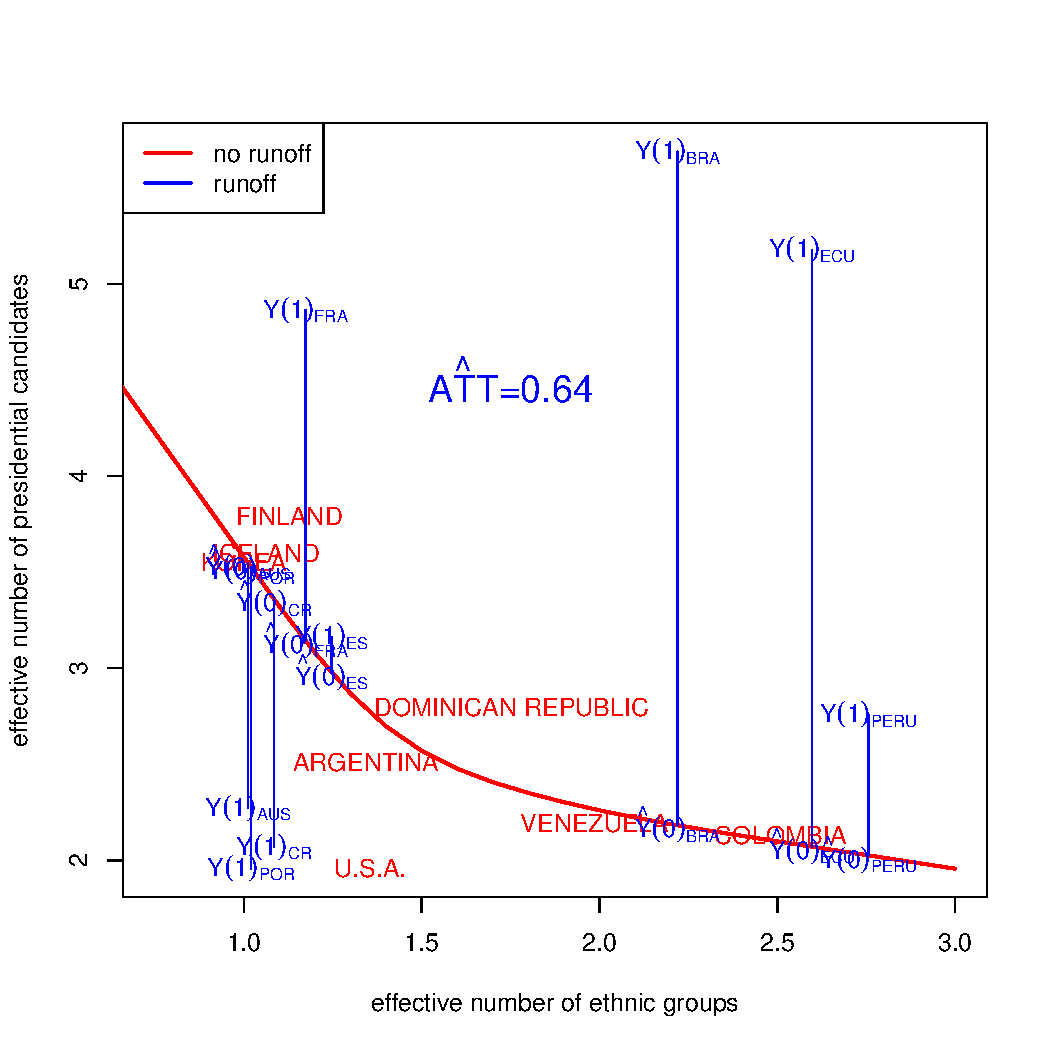
\includegraphics[height=3in]{figures/p15c.pdf}
%  \end{center}
%  \vspace{-0.275in}
%\end{figure}
%
%}
%








%\frame{
%
%Then considering the bivariate CEF, by definition:
%$$
%\E[Y| X = x] = \left\{
%     \begin{array}{lr}
%            \E[Y | X = 0]  & : x = 0 \\
%       \E[Y | X = 1] & : x = 1
%     \end{array}
%   \right.
%   $$
%
%}
%
%\frame{
%
%Then we can {\it definitionally} write $\E[Y| X]$ as a linear function of $X$.
%$$
%\E[Y| X] = \beta_0 + \beta_1 X,
%$$
%where
%\begin{itemize}
%\item $\beta_0 =  \E[Y | X = 0] $
%\item $\beta_1 =  \E[Y | X = 1] - \E[Y | X = 0]$.
%\end{itemize}
%
%}
%
%\frame{
%
%We could define an alternative specification that is logically equivalent. Consider the regression {\it without an intercept}:
%$$
%\E[Y| X] = \gamma_1(1 - X) + \gamma_2 X,
%$$
%where
%\begin{itemize}
%\item $\gamma_1 =  \E[Y | X = 0] $
%\item $\gamma_2 =  \E[Y | X = 1]$.
%\end{itemize}
%
%}
%
%\frame{
%
%When $X$ is binary, the CEF {\it must be} the BLP.
%
%\vspace{0.2in}
%
%The regression estimates of the $\beta$s can be written {\it just using} conditional means.
%
%}
%
%
%
%
%\frame{
%
%The idea generalizes to the multivariate case.
%
%}
%
%\frame{
%
%Consider binary $X_1$, $X_2$:
%
%$$
%\E[Y| X_1 = x_1, X_2 = x_2] = \left\{
%     \begin{array}{lr}
%            \E[Y | X_1 = 0, X_2 = 0]  & : x_1 = 0, x_2 = 0 \\
%            \E[Y | X_1 = 1, X_2 = 0]  & : x_1 = 1, x_2 = 0 \\
%            \E[Y | X_1 = 0, X_2 = 1]  & : x_1 = 0, x_2 = 1 \\
%            \E[Y | X_1 = 1, X_2 = 1]  & : x_1 = 1, x_2 = 1
%     \end{array}
%   \right.
%   $$
%
%}
%
%\frame{
%
%Then we can {\it definitionally} write $\E[Y| X_1, X_2]$ as a linear function of $X_1$, $X_2$ and $X_1 X_2$.
%
%$$
%\E[Y  | X_1, X_2] = \beta_0 + \beta_1 X_1 + \beta_2 X_2 + \beta_3 X_1 X_2
%$$
%where
%\begin{itemize}
%\item $\beta_0 =  \E[Y | X_1 = 0, X_2 = 0]  $
%\item $\beta_1 =   \E[Y | X_1 = 1, X_2 = 0]  -   \E[Y | X_1 = 0, X_2 = 0] $
%\item $\beta_2 =   \E[Y | X_1 = 0, X_2 = 1]  -   \E[Y | X_1 = 0, X_2 = 0] $
%\item $\beta_3 =   \E[Y | X_1 = 1, X_2 = 1]  - \E[Y | X_1 = 1, X_2 = 0]  - \E[Y | X_1 = 0, X_2 = 1] - \E[Y | X_1 = 0, X_2 = 0]$
%\end{itemize}
%
%}
%
%
%\frame{
%
%Logically equivalent, using indicator or ``dummy" variables:
%
%\begin{align*}
%\E[Y  | X_1, X_2]  = & \gamma_1 \I[X_1 = 0, X_2 = 0]  + \gamma_2 \I[X_1 = 1, X_2 = 0] +\\
%& \gamma_3 \I[X_1 = 0, X_2 = 1] + \gamma_4 \I[X_1 = 1, X_2 = 1]
%\end{align*}
%where
%\begin{itemize}
%\item $\gamma_1 =  \E[Y | X_1 = 0, X_2 = 0]  $
%\item $\gamma_2 =   \E[Y | X_1 = 1, X_2 = 0]  $
%\item $\gamma_3 =   \E[Y | X_1 = 0, X_2 = 1]  $
%\item $\gamma_4 =   \E[Y | X_1 = 1, X_2 = 1]  $
%\end{itemize}
%
%}
%
%\frame{
%
%These are cases of {\it saturated models}: when every unique combination of values of the explanatory variables is included in a fully flexible way. This is only possible with {\it discrete} regressors ($X$ variables).
%
%\vspace{0.2in}
%
%This means including dummy variables for every possible value of each variable, and all possible (including multiway) interactions. Or just dummy variables for each unique combination, and excluding the intercept.
%
%\vspace{0.2in}
%
%With a saturated model, the CEF is, by definition, the BLP.
%
%}
%
%
%
%
%
%
%\frame{
%
%Remaining ``non-linear'' issues with a single $X$:
%\begin{itemize}
%\item How to choose the degree of the polynomial?
%\item What if not linear in $\beta$?
%\item statistical/machine learning approaches
%\item what if $X$ is ordinal?
%\end{itemize}
%
%}

%\frame{
%How to choose the degree of the polynomial?
%\begin{itemize}
%\item Sieve Estimation:\\
%Choose the degree of the polynomial to be $K_n = \ceil{n^{1/9}}$
%\item Cross-validation:\\
%\begin{enumerate}
%\item Separate data into $G$ groups
%\item Leave one group out as test data
%\item fit model using remaining groups
%\item calculate prediction error on test data
%\item repeat for all $G$ groups
%\item repeat whole process for many different polynomials and choose best based on test data prediction error
%\end{enumerate}
%\end{itemize}
%
%}
%
%\frame{
%Leave one out CV
%
%\begin{itemize}
%\item $G=n$ (each observation is a group)
%\item test error easy to calculate for OLS (includes polynomial models)
%$$
%\frac{1}{n}\sum_{i=1}^n\frac{(y_i - \hat y_i)^2}{(1-h_i)^2}
%$$
%\end{itemize}
%
%}
%
%\frame{
%
%Examples of nonlinear in $\beta$
%
%\begin{align*}
%g(X) &= e^{\beta_0 + \beta_1 X}\\
%g(X) &= \frac{e^{\beta_0 + \beta_1 X}}{1 + e^{\beta_0 + \beta_1 X}}
%\end{align*}
%
%How to fit?
%
%\vsf
%
%How to interpret?
%%$$\frac{\partial g(X)}{\partial X} = ?$$
%
%}








\end{document}